\chapter{System architecture}
Since the library is based on the client-server architectural pattern, its functionalities are split in two distinct modules:
\begin{itemize}
	\item \textit{Client module} - It provides the features required to connect and communicate with a game server. In particular, it allows the client side developer to create rooms (that will be hosted on the server) and to perform operations on them (e.g. join, leave, message...).
	\item \textit{Server module} - It internally implements the logic to handle clients connections and it allows the developer to run a gameserver and to define new types of room. Moreover, it contains all the logic to handle matchmaking requests too.
\end{itemize}

Client and server modules are not fully separated but, on the contrary, they share some common concepts like communication protocol and data serialization utilities required when parsing data received and sent through the network.
\\
A common notion of room is the most important concept that clients and server must agree to. That is decribed in section \ref{room-arch}.

\section{Room} \label{room-arch}


\begin{figure}[H]
	\centering
	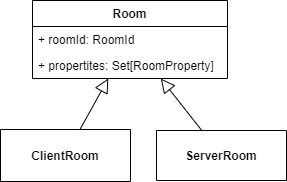
\includegraphics[scale=0.7]{images/3-architecture/room-class-3.png}
	\caption{Room class diagram}
	\label{fig:room_classes}
\end{figure}


At the most abstract level, a room is an entity that owns an unique Id and some properties that describe the room itself (figure \ref{fig:room_classes}).
\\
This is the basic model shared between clients and server that each model will extend.

\bigskip
\textit{ServerRoom}
\\
The server room is the one that will be used by the server side developer. It provides functionalities to communicate and interact with connected clients. Besides, as specified in server requirement 2.1, the room behavior can be defined by the developer according to the application custom logic.

\bigskip
\textit{ClientRoom}
\\
On the other hand, the client room is the room that a client side developer will use. This component is meant to provide an interface towards the server side room, so that the developer can both send and receive messages from it. Obviously, it exposes functionalities to define custom behavior too, as specified in client requirement 9.

\section{Server architecture} \label{sec:server_arch}
The main components of the server side architecture are visible in figure \ref{fig:server_classes}. 

\begin{figure}[H]
	\centering
	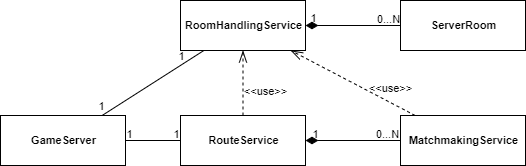
\includegraphics[scale=0.7]{images/3-architecture/server-architecture.png}
	\caption{Server architecture}
	\label{fig:server_classes}
\end{figure}

\bigskip
\textit{GameServer}
\\
The \texttt{GameServer} is the core component of the architecture and the starting point from where all the other components are created.
When dealing with the server module, a developer will mostly make use of its interface.

As shown in figure \ref{fig:server_classes}, it is connected to two other components: the \texttt{RouteService} and the \texttt{RoomHandlingService}.

\bigskip
\textit{RoomHandlingService}
\\
As the name suggests, the \texttt{RoomHandlingService} is the component used to manage rooms. It is meant to:
\begin{itemize}
	\item Keep track of which rooms are currently active in the system
	\item Provide a way to interact with rooms (e.g creating and deleting rooms)
	\item Provide a way to define admissible types of room.
\end{itemize}

\bigskip
\textit{RouteService}
\\
This service is the classic routing module.
Every client request received by the gameserver using the request-response pattern is served by this component.
It defines routes (and associated handlers) that clients should contact when interacting with the server.
\\
Client requests can basically be split in two types:
\begin{itemize}
	\item Requests concerning rooms (e.g. connect to a room or retrieve available rooms). These requests are directly satisfied by the helping of the \texttt{RoomHandlingService}.
	\item Requests concerning matchmaking (e.g. join a matchmaking queue). These requests are forwarded and delegated to the right \texttt{MatchmakingService}, depending on the room type.
\end{itemize}

\bigskip
\textit{MatchmakingService}
\\
The \texttt{MatchmakingService} is the component that implements the matchmaking logic for a given type of room (i.e. adding clients to a queue, and eventually create fair groups according to some information about such clients). It needs to interact with the \texttt{RoomHandlingService} since, when a group of clients is formed, it must be created a room where those clients should connect to.


\section{Client Architecture}

Class diagram of client side architecture is shown in figure \ref{fig:client_architecture}. 
\begin{figure}[H]
	\centering
	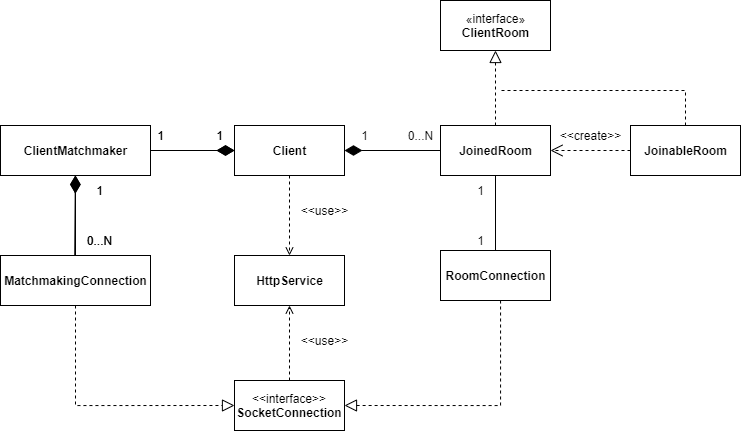
\includegraphics[scale=0.65]{images/3-architecture/client-architecture.png}
	\caption{Client architecture diagram}
	\label{fig:client_architecture}
\end{figure}
\bigskip
\textit{Client}
\\
\texttt{Client} class is the main access to client side functionalities.
It exposes three main capabilities, namely:
\begin{itemize}
  \item It handles few operations on rooms (e.g. to retrieve or create rooms) by exploiting the \texttt{HttpService}.
  \item It keeps track of joined rooms.
  \item It enables the access to client side matchmaker.
\end{itemize}

\bigskip
\textit{HttpService}
\\
\texttt{HttpService} is the module that handles http communication to the game server. It provides two main functionalities, that is:
\begin{itemize}
  \item It makes http requests to the server (Get, Post).
  \item It allows the opening for websocket connections.
\end{itemize}

\bigskip
\textit{ClientMatchmaker}
\\
 \texttt{ClientMatchmaker} is the component that provides the matchmaking functionalities for clients (e.g. to join or leave matchmaking queues). It keeps a websocket connection (\texttt{MatchmakingConnection}) opened to a server side matchmaker for each queue joined by the client.

\bigskip
\textit{ClientRoom}
\\
A \texttt{ClientRoom} represents an instance of a room from the client's perspective. A room is ``joinable'' at first  (\texttt{JoinableRoom}), meaning that a client can join or reconnect to such room. 
Then, when a room is accessed, it becomes ``joined'' (\texttt{JoinedRoom}). At this point, a websocket connection (\texttt{RoomConnection}) with the server side room is opened to enable the communication between the two sides.


\section{Client-Server Interaction}
The requirements analysis led to the definition of three types of interaction between client and server:
\begin{enumerate}
	\item Client to GameServer \\
	This interaction takes place in those situations where the client makes a request to the server and waits for a specific response: for example, getting the list of all rooms that can be joined. Such requests are based on the classical request-response pattern and will be handled by the definition of a REST protocol as shown in table
	 \ref{table:server_routes}.
	\begin{table}[]
		\begin{tabular}{p{2cm}p{4cm}p{2cm}p{5.5cm}}
			\textbf{Http Method} & \textbf{Path}	  & \textbf{Payload}  & \textbf{Result}                                                            		\\\\
			GET                  & /rooms             & filters           & get all the rooms that match the filters in the payload                        	\\\\
			GET                  & /rooms/:type       & filters           & get all the rooms with the given type (filtered by the payload)     	\\\\
			GET                  & /rooms/:type/:id   & empty             & get the room with the given Id, searching among rooms of the given type         	\\\\
			POST                 & /rooms/:type       & options           & create a room of the given type with the options (i.e. properties to be set) passed in the payload          	\\\\
			GET                  & /connection/:id    & websocket request & open a web socket connection with the room that has the given Id               	\\\\
			GET                  & /matchmaking/:type & websocket request & open a web socket with the matchmaking service relative to the given room type 	\\\\
		\end{tabular}
		\caption{\label{table:server_routes} \textit{Server REST protocol for request-response interaction}}
	\end{table}
	\item  Client to Room \\
	In this case, we are in a situation where a client wants to establish a connection with a given a room in order to both send and receive messages. Since the server could send data to the client not just in front of an explicit client request (for example, on message broadcasting), the communication requires a full-duplex communication channel.
	
	The chosen solution is the usage of websockets protocol since it provides the exact described behavior. Specifically, when a client wants to interact with a room, a websocket between that client and the server is created, and then, messages exchanged from the first and the room flow through such socket.
	
    The socket will be then closed when the client ends his interaction with the room (few scenarios are possible: e.g. failed join, room leaving, timeout kicking out).

 	As well as protocol messages required to handle lifecycle (e.g. joining, leaving),  clients can send custom messages once they joined the room. This means that a generic serialization format the developer can adhere to is required.
	
	
	\item Client to Matchmaking \\
	The last type of interaction is the one that takes place when a client is interacting with a matchmaking service. Websockets are used here too since another full-duplex channel is required. Indeed, when a client sends a request in order to join the matchmaking queue, the server response is not immediate, and the communication must be kept open until the matchmaking service will eventually create a group of clients. Only then the server will respond to the client with a message that contains some information required to join the room that will host the game.
	In the end, since a matchmaking service is associated with a specific type of room, the client could have multiple sockets open in parallel with different matchmaking services.
\end{enumerate}









